\subsection{Диаграмма классов}
	\begin{figure}[H]
		\centering
		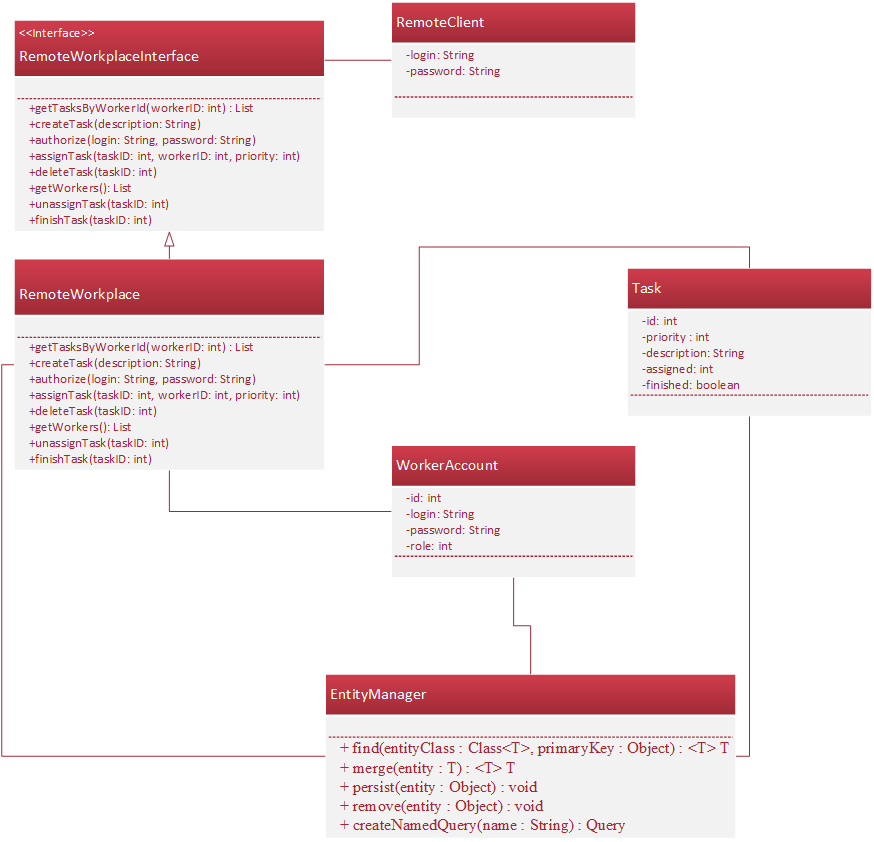
\includegraphics[width=1\textwidth]{../materials/ClassDiagram.png}
		\caption{Диаграмма классов проекта}
		\label{fig:ClassDiag}
	\end{figure}
	
\subsection{Описание классов бизнес-логики}
	\begin{itemize}
		\item Класс <<RemoteWorkplace>>
			\begin{itemize}
					 
				\item \textit{List<Task> getTasksByWorkerId(int workerID)} - возвращает список задач работника в порядке убывания приоритета (если $workerID=-1$, то список свободных задач).
				
				\item \textit{createTask(description: String)} - создает задачу
				
				\item \textit{String authorize(login: String, password: String)} - авторизация, возвращает идентификатор сессии
				
				\item \textit{assignTask(taskID: int, workerID: int, priority: int) } - назначить задачу работнику с выставлением приоритета.
				
				\item \textit{deleteTask(taskID: int)} - удалить задачу
				
				\item \textit{getWorkers(): List} - список всех работников
				
				\item \textit{unassignTask(taskID: int)} - снять задачу с работника
								
				\item \textit{finishTask(taskID: int)} - отметить задачу, как выполненную 
				
			\end{itemize}	
		\item Класс <<EntityManager>>
		\begin{itemize}
			
			\item \textit{T merge(entity : T)} - синхронизировать состояние объекта с базой данных при изменении. Возвращает синхронизированный объект
			
			\item \textit{persist(entity : Object)} - синхронизировать состояние объекта с базой данных (например, при добавлении).
			
			\item \textit{remove(entity : Object)} - удалить объект из БД
			
			\item \textit{createNamedQuery(name : String)} - создать SQL-запрос к базе данных		
		\end{itemize}		
		
		\item Класс <<WorkerAccount>>
		\begin{itemize}
			
			\item \textit{int id} - идентификатор пользователя
			\item \textit{String login} - логин
			\item \textit{String password} - пароль
			\item \textit{String firstName} - имя
			\item \textit{String lastName} - фамилия
			\item \textit{String session} - текущая сессия
			\item \textit{int role} - тип аккаунта (1 - менеджер, 2 - работник)	
		\end{itemize}	
		
		\item Класс <<Task>>
		\begin{itemize}
			
			\item \textit{int id} - идентификатор задачи
			\item \textit{int priority} - приоритет задачи
			\item \textit{String description} - описание задачи
			\item \textit{int assigned} - id назначенного работника, по умолчанию -1
			\item \textit{boolean finished} - выполнена ли задача
		\end{itemize}
\end{itemize}	